\chapter{FOPT5 - Eigenständige Client-Server-Anwendungen in Java (Programmierung verteilter Anwendungen 1)}

\section{Lehrstoff}

Das Skript FOPT5 bezieht sich auf folgende Inhalte im Buch:

\begin{tcolorbox}[colback=white!20,color=white]
    \begin{enumerate}
        \setcounter{enumi}{0}
        \item \textbf{Einleitung und Grundlagen von Rechnernetzen}
        \begin{itemize}
            \item[] Kapitel 5
            \item[] Abschnitt 5.1
        \end{itemize}

        \item \textbf{Socket-Schnittstelle}
        \begin{itemize}
            \item[] Abschnitt 5.2
        \end{itemize}

        \item \textbf{Kommunikation über UDP mit Java-Sockets}
        \begin{itemize}
            \item[] Abschnitt 5.3
        \end{itemize}

        \item \textbf{Multicast-kommunikation mit Java-Sockets}
        \begin{itemize}
            \item[] Abschnitt 5.4
        \end{itemize}

        \item \textbf{Kommunikation über TCP mit Java-Sockets}
        \begin{itemize}
            \item[] Abschnitt 5.5
        \end{itemize}

        \item \textbf{Sequenzielle und parallele Server}
        \begin{itemize}
            \item[] Abschnitt 5.6
            \item[] Abschnitt 5.6.1
            \item[] Abschnitt 5.6.2
            \item[] Abschnitt 5.8
            \item[] optional: 5.6.3, 5.6.4, 5.7
        \end{itemize}

        \item \textbf{Prinzip von RMI}
        \begin{itemize}
            \item[] Kapitel 6
            \item[] Abschnitt 6.1
        \end{itemize}

        \item \textbf{Einführendes RMI-Beispiel}
        \begin{itemize}
            \item[] Abschnitt 6.2
        \end{itemize}

        \item \textbf{Parallelität bei RMI-Methodenaufrufen}
        \begin{itemize}
            \item[] Abschnitt 6.3
        \end{itemize}
    \end{enumerate}
\end{tcolorbox}

\begin{tcolorbox}[colback=white!20,color=white]
    \begin{enumerate}
        \setcounter{enumi}{9}
    \item \textbf{Wertübergabe für Parameter und Rückgabewerte}
    \begin{itemize}
        \item[] Abschnitt 6.4
    \end{itemize}

    \item \textbf{Referenzübergabe für Parameter und Rückgabewerte}
    \begin{itemize}
        \item[] Abschnitt 6.5
    \end{itemize}

    \item \textbf{Transformation lokaler in verteilte Anwendungen}
    \begin{itemize}
        \item[] Abschnitt 6.6.1
        \item[] Abschnitt 6.6.3
    \end{itemize}

    \item \textbf{Verschiedenes}
    \begin{itemize}
        \item[] Abschnitt 6.10
        \item[] optional: 6.7, 6.8, 6.9
    \end{itemize}
    \end{enumerate}
\end{tcolorbox}

\newpage

\section{Socket-Schnittstelle}

Die \textbf{Socket-Schnittstelle} ermöglicht die Kommunikation von verteilten Client-Server-Anwendungen untereinander.

\begin{tcolorbox}[enlarge top by=0.5cm,enlarge bottom by=0.5cm]
Die Socket-Schnittstelle stellt eine Schnittstelle zwischen \textbf{Schicht 4} (Transportschicht) und \textbf{Schicht 5} (Anwendungsschicht) dar.
\end{tcolorbox}

\subsection{Socket-Schnittstelle zu UDP}

Eine Schnittstelle zu \textbf{UDP} ist relativ einfach zu realisieren, da hier keine Operationen für den Verbindungsauf- und -abbau nötig sind $\rightarrow$ es sind nur Operationen für das Senden und Empfangen notwendig.\\

\noindent
Bei der Erzeugung eines \textbf{Sockets} kann eine Portnummer angegeben werden, für gesendete Nachrichten ist das dann die \textbf{Quellportnummer} der Nachricht.\\
Der Socket empfängt nur Nachrichten, die an diesen Port adressiert wurden.\\

\noindent
Bei \textbf{Client/Server-Anwendungen} geht die Initiative vom Client aus, der eine Anfrage an einen Server schickt.\\
Der Server antwortet an die in der Nachricht enthaltenen IP-Adresse und Quellportnummer.

\begin{tcolorbox}[enlarge top by=0.5cm,enlarge bottom by=0.5cm]
I.d.R verwendet ein Client eine beliebige freie Portnummer.\\

\noindent
Dienste laufen auf Servern auf wohlbekannten Portnummern, bspw. ``https`` auf Port $443$\footnote{
s. a. ``Hypertext Transfer Protocol Secure``: \url{https://de.wikipedia.org/wiki/Hypertext_Transfer_Protocol_Secure} - abgerufen 30.01.2024
}.\\
Ein Server, der unter einer bestimmten Portnummer laufen soll, kann nur gestartet werden, wenn die Portnummer nicht schon belegt ist.
\end{tcolorbox}\\

\newpage
\noindent
Beispiel für eine Programmstruktur für eine Kommunikation zwischen UDP-Client und -Server:
\begin{minted}[mathescape,

    numbersep=5pt,
    gobble=2,
    frame=none,
    framesep=2mm]{java}
    // UDP Client
    c = ErzeugeUDPSocket();
    while (beliebig) {
        sende Nachricht über Socket c an ServerAdresse/Portnummer;
        warte auf Nachricht an Socket c;
        tue etwas mit der Nachricht;
    }

    // UDP Server
    s = ErzeugeUDPSocketAnPort(port);
    while (beliebig) {
        warte auf Nachricht von Client an Socket s;
        analysiere die Nachricht;
        führe Aktion aus;
        schicke über s Antwort an die Adresse/Portnummer der Nachricht;
    }
\end{minted}

\begin{tcolorbox}[enlarge top by=0.5cm,enlarge bottom by=0.5cm]
    Die Portnummern für \textbf{TCP} und \textbf{UDP} existieren unabhängig voneinander: Ist ein Port $n$ für TCP reserviert, kann die gleiche Portnummer trotzdem für UDP verwendet werden.
\end{tcolorbox}

\subsection{Socket-Schnittstelle zu TCP}

Die Besonderheit bei TCP ist, dass der Server auf einen Port auf eine Anfrage (über einen Socket) wartet, und dann mit dem Client die Kommunikation über einen neuen Socket realisiert (s. Abbildung~\ref{fig:tcpsockets}).\\

\begin{figure}
    \centering
    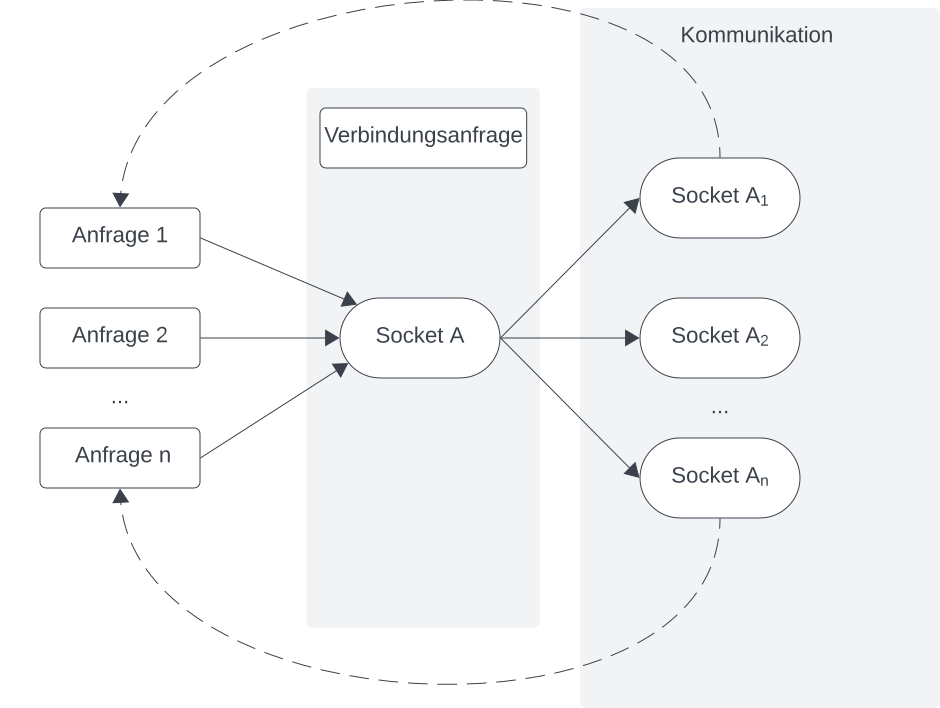
\includegraphics[scale=0.5]{chapters/fopt5/img/sockets/tcpsockets}
    \caption{Von einem TCP-Socket angenommene Verbingungsanfragen führen zu neuen Sockets, die letztendlich für die Kommunikation mit den Clients verantwortlich sind.
    Nach Verbindungsabbruch werden diese Sockets verworfen, der Socket zur Verbindungsannahme wird weiterverwendet(Quelle: eigene)}
    \label{fig:tcpsockets}
\end{figure}



\noindent
$\rightarrow$ für einen Port kann es somit mehrere Sockets geben.\\


\noindent
Beispiel für eine Programmstruktur für eine Kommunikation zwischen UDP-Client und -Server:
\begin{minted}[mathescape,
    numbersep=5pt,
    gobble=2,
    frame=none,
    framesep=2mm]{java}
    // TCP Client
    c = ErzeugeTCPSocket();
    baue über c eine Verbindung zu ServerAdresse/Portnummer auf;
    /* c ist blockiert, bis Timeout abgelaufen oder Anfrage angenommen */
    while (beliebig) {
        sende Nachricht über Socket c;
        warte auf Nachricht an Socket c;
        tue etwas mit der Nachricht;
    }
    schliesse die Verbindung über c;

    // TCP Server
    s = ErzeugeTCPSocketAnPort(port);
    while (beliebig) {
        warte auf Verbindungsanfrage an s und erstelle
        neuen Socket q bei neuer Verbindung;

        while (Verbindung besteht) {
            warte auf Nachricht von Client an Socket q
            wenn nachricht da ist {
                analysiere die Nachricht;
                führe Aktion aus;
                schicke über q Antwort an die Adresse/Portnummer
                der Nachricht;
            } ansonsten nach timeout oder verbindungsabbruch {
                schliesse Verbindung über q;
                verlasse die innere schleife und warte auf
                neue verbindung;
            }

        }
    }
\end{minted}\\

\noindent
Es gibt bei \textbf{TCP} höchstens eine Verbindung von einem Port auf einem Rechner zu einem anderen Port auf einen anderen Rechner, aber es können mehrere Verbindungen von einem Port zu unterschiedlichen Ports des Zielrechners existieren, bzw. es kann ein Rechner mehrere Verbindungen zu einem bestimmten Port auf einem unterschiedlichen Zielrechner erstellen (s. Abbildung~\ref{fig:tcpconnections}).


\begin{figure}
    \centering
    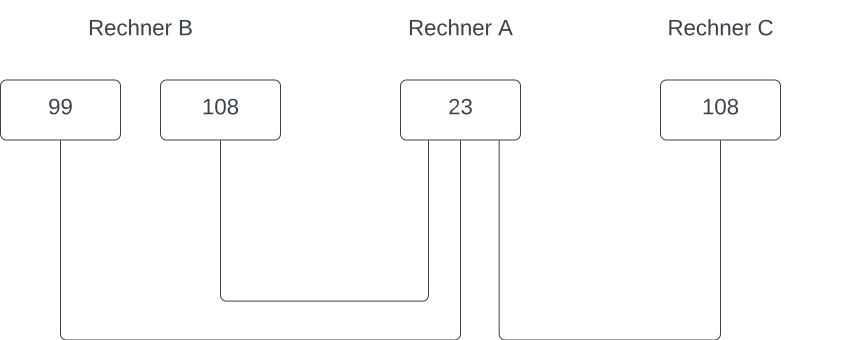
\includegraphics[scale=0.5]{chapters/fopt5/img/sockets/tcpconnections}
    \caption[fontsize=\small]{Rechner $A$ bedient zweimal dieselbe Portnummer $108$ auf zwei unterschiedlichen Rechnern $B$ und $C$, von Port $23$ aus. Gleichzeitig wird Port $99$ von Rechner $B$ von Rechner $A$ bedient. (Quelle: in Anlehnung an \cite[265, Bild 5.3]{Oec22})}
    \label{fig:tcpconnections}
\end{figure}


\subsection{Socket-Schnittstelle für Java}

Die Java-Klassenbibliothek enthält u.a. im Package \code{java.net} Implementierung zur Realisierung von Socket-Kommunikation.\\

\noindent
\code{InetAddress} ist eine Klasse zur Handhabung von von Rechnernamen / IP-Adressen.\\

\noindent
\code{DatagramPacket} und \code{DatagramSocket} werden zur \textbf{UDP}-Kommunikation verwendet.\\

\noindent
\code{Socket} und \code{ServerSocket} werden zur \textbf{TCP}-Kommunikation benötigt.


\section{Kommunikation über UDP mit Java Sockets}

\code{DatagramPacket} wird mit der IP-Adresse und Portnummer des Partners konfiguriert $\rightarrow$ für zu sendende Pakete ist das die Ziel-Adresse und Ziel-Portnummer, für empfangene Pakete ist das die Quelladresse und Quell-Portnummer.\\

\noindent
Ein \code{DatagramPacket} repräsentiert Daten in Form eines Feldes des Typs \code{byte} und einer Länge, die höchstens so groß sein kann wie die Feldlänge - ist die Länge kleiner als die Feldlänge, wurde nur die angegebene Länge als relevant betrachtet.\\

\noindent
Server verwenden für die Kommunikation bei der Erzeugung von \code{DatagramSocket} i.d.R. eine feste Portnummer, auf der der Service laufen soll.\\
Clients verwenden i.d.R. den parameterlosen Konstruktor, ein freier Port wird dann zugeteilt.

\begin{minted}[mathescape,
    numbersep=5pt,
    gobble=2,
    frame=none,
    framesep=2mm]{java}
    public class DatagramPacket {
        public DatagramPacket(byte[] buf, int length) {...}
        public DatagramPacket(
            byte[] buf, int length, InetAddress address, int port) {...}
        ...
    }

    public class DatagramSocket implements Closeable {
        public DatagramSocket() throws SocketExcpetion {...}
        public DatagramSocket(int port) throws SocketExcpetion {...}
        public send(DatagramPacket p) throws IOExcpetion {...}
        public receive(DatagramPacket p) throws IOExcpetion {...}
        ...
    }
\end{minted}\\

\noindent
Die Methode \code{receive()} eines Sockets ist \texbf{blocking}, es wird so lange gewartet, bis eine Nachricht eintrifft, oder ein durch \code{setSoTimeout(int timeout)} angegebener Timeout eintritt.\\

\noindent
Mit \textbf{try-with-resources}\footnote{
    ``The try-with-resources Statement``: \url{https://docs.oracle.com/javase/tutorial/essential/exceptions/tryResourceClose.html} - abgerufen 31.01.2024
} kann ein Socket automatisch geschlossen werden.

\begin{tcolorbox}[enlarge top by=0.5cm,enlarge bottom by=0.5cm]
Ein Objekt, dessen Klasse \code{AutoCloseable} implementiert, kann als \textit{Resource} für das \textit{try-with-resource}-Statement genutzt werden.
Das schliesst auch Objekte ein, deren Klasse \code{Closeable} implementiert, da \code{Closeable} von \code{AutoCloseable} abgeleitet ist.\\

\noindent
Wenn \code{AutoCloseable}-Objekte weder mit \textbf{try-with-resources} noch mit \code{close} verwendet werden, gibt der Compiler seit Java 7 eine Warnung aus.\\

\noindent
Ein \code{try-with-resources}-Statement kommt ohne \code{catch}-Block aus.\\
Wenn die Konstruktoren der erzeugten Objekte eine Exception werfen, sollte das in der Methoden-Signatur angegeben werden, oder ein \code{catch}-Block sollte verwendet werden.
\end{tcolorbox}

\begin{minted}[mathescape,
    numbersep=5pt,
    gobble=2,
    frame=none,
    framesep=2mm]{java}
    try (DatagramSocket updSocket = new DatagramSocket(1234);
     PrintWriter pw = new PrintWriter("foo.txt");) {
        ...
    } catch (SocketException | FileNotFoundException e) {
        ...
    }
\end{minted}\\

\section{Multicast-Kommunikation mit Java-Sockets}
Mittels der Klasse \code{MulticastSocket} (abgeleitet von \code{DatagramSocket}) kann sich ein Socket mittels der Methode \code{joinGroup()} auf eine \textbf{Multicast-Adresse} aufschalten.\\
Der Socket erhält so jede Nachricht, die an diese Adresse geschickt wurde.\\
Mittels \code{leaveGroup()} schaltet sich der Socket von dem Nachrichtenempfang wieder ab.

\begin{tcolorbox}[enlarge top by=0.5cm,enlarge bottom by=0.5cm]
\textbf{IP-Multicast-Adressen} sind spezielle Adressen, mit denen mehr als ein Rechner angesprochen werden kann.\\
Für \textbf{IPv4} ist hierfür der Bereich $224.0.0.0 - 239.255.255.255$ reserviert\footnote{
s.a. ``Multicast address``: \url{https://en.wikipedia.org/wiki/Multicast_address} - abgerufen 31.01.2024
}.
\end{tcolorbox}

\noindent
Zum Senden von Nachrichten an eine Multicast-Adresse reicht ein \code{DatagramSocket}.\\
Will man aber einen \textbf{TTL}\footnote{\textit{Time-to-Live} - auch \textbf{hop limit} - wird verwendet, um ein Datenpaket mit einer max. Lebensdauer zu konfigurieren, was verhindern soll, dass Datenpakete unendlich lange in einem Netzwerk existieren. S. a. \url{https://en.wikipedia.org/wiki/Time_to_live} - abgerufen 31.01.2024}-Wert angeben, muss ein \code{MulticastSocket} verwendet werden.

\blockquote[{`DARPA INTERNET PROGRAM PROTOCOL SPECIFICATION`: \url{https://datatracker.ietf.org/doc/html/rfc791#section-1.4} - abgerufen 31.01.2024}]{
    The Time to Live is an indication of an upper bound on the lifetime of an internet datagram. It is set by the sender of the datagram and reduced at the points along the route where it is processed. If the time to live reaches zero before the internet datagram reaches its destination, the internet datagram is destroyed. The time to live can be thought of as a self destruct time limit.
}

\section{Kommunikation über TCP mit Java-Sockets}


Für \textbf{TCP}-Kommunikation werden in Java die Klassen \code{Socket} und \code{ServerSocket} eingesetzt.\\

\noindent
Der \textbf{Client} erzeugt ein \code{Socket}-Objekt unter Angabe der Adresse, zu der sich der Client verbinden möchte.\\

\noindent
Der \textbf{Server} nutzt die Klasse \code{ServerSocket}, der über \code{accept()} auf eingehende Verbindungen wartet.\\
Eine Verbindung wird von \code{accept()} über einen zurückgegebenen \code{Socket} signalisiert, der dann für die Kommunikation mit dem Client genutzt werden kann (s.a. Abbildung~\ref{fig:tcpsockets}).\\

\noindent
Eine \textbf{TCP}-Verbindung kann als zwei unidirektionale Verbindungen gesehen werden (Eingabe, Ausgabe).\\
$\rightarrow$ Es gibt deshalb nicht nur die Möglichkeit, mit \code{close()} der Klasse \code{java.net.Socket} die Verbindung komplett zu schließen, sondern es gibt darüber hinaus noch die Möglichkeiten, die Eingangs-/Ausgangsverbindungen getrennt voneinander zu schließen:


\begin{itemize}
    \item \code{shutdownInput()} $\rightarrow$ weiter senden, nicht mehr empfangen: ``Any data sent to the input stream side of the socket is acknowledged and then silently discarded.``\footnote{``Class Socket``: \url{https://docs.oracle.com/en/java/javase/21/docs/api/java.base/java/net/Socket.html#shutdownInput()} - abgerufen 31.01.2024
    }
    \item \code{shutdownOutput()} $\rightarrow$ weiter empfangen, nicht mehr senden.\footnote{``If you write to a socket output stream after invoking shutdownOutput() on the socket, the stream will throw an IOException.`` s. \url{https://docs.oracle.com/en/java/javase/21/docs/api/java.base/java/net/Socket.html#shutdownOutput()} - abgerufen 31.01.2024
    }
\end{itemize}

\noindent
\code{Socket} bietet keine Methoden zum Schreiben/Lesen {bzw.} Senden und Empfangen (vgl.~\cite[282]{Oec22}), stattdessen nutzt man die über \code{getInputStream()} / \code{getOutputStream()} zur Verfügung gestellten \textbf{Byteströme}.

\begin{tcolorbox}[enlarge top by=0.5cm,enlarge bottom by=0.5cm]
    \begin{itemize}
        \item \textbf{InputStream} / \textbf{OutputStream}: byteweise Ein-/Ausgabe
        \item \textbf{Reader} / \textbf{Writer}: zeichenweise Ein-/Ausgabe
    \end{itemize}
\end{tcolorbox}

\noindent
$\rightarrow$ über \textit{Adapter}/\textit{Dekorierer} kann man diese Byteströme direkt zum Lesen/Senden von \code{String}s nutzen.\\
I.d.R. sollte man hierfür Puffer nutzen die \textit{geflushed}\footnote{alles, was sich im Buffer befindet, wird an den darunterliegenden Ausgabestrom gesendet} werden, wenn sie voll sind, damit nicht für jedes einzelne Zeichen Betriebssystemaufrufe stattfinden müssen.\\

\noindent
Da \textbf{TCP} datenstromorientiert ist, kann man Trennzeichen zum Markieren von Nachrichtengrenzen nutzen.
Hierzu verwendet man in der Regel eine \textit{newline}, also \textbf{\textbackslash n}.

Beispiel für das Senden von Daten über einen Socket mittels eines \code{BufferedWriter}s\footnote{
    ``Class BufferedWriter``: \url{https://docs.oracle.com/en/java/javase/21/docs/api/java.base/java/io/BufferedWriter.html} - abgerufen 31.01.2024
}:
\begin{minted}[mathescape,
    numbersep=5pt,
    gobble=2,
    frame=none,
    framesep=2mm]{java}
    OutputStrean os = socket.getOutputStream();
    OutputStreamWriter ow = new OutputStreamWriter(os);
    BufferedWriter bw = new BufferedWriter(ow);
    ...
    bw.write("message");
    bw.newline();
    bw.flush();
\end{minted}\\

Beispiel für das Lesen von Daten über einen Socket mittels eines \code{BufferedReader}s\footnote{
    ``Class BufferedReader``: \url{https://docs.oracle.com/en/java/javase/21/docs/api/java.base/java/io/BufferedReader.html} - abgerufen 31.01.2024
}:
\begin{minted}[mathescape,
    numbersep=5pt,
    gobble=2,
    frame=none,
    framesep=2mm]{java}
    InputStream is = socket.getInputStream();
    InputStreamReader ir = new InputStreamReader(is);
    BufferedReader bw = new BufferedReader(ir);
    ...
    String message = br.readLine();
\end{minted}\\

\noindent
Das Ende eines Datenstroms wird durch den Rückgabewert \code{null} angezeigt (bei Dateioperationen {bspw.} als Ende der Datei; TCP-Verbindung: Client hat die Verbindung geschlossen usw.).

\begin{tcolorbox}[enlarge top by=0.5cm,enlarge bottom by=0.5cm]
    Das Lesen ist eine blockierende Operation.\\
    Das Schreiben von Daten mit anschliessendem \code{flush()} ist nicht blockierend.
    Sollte der Sender allerdings direkt nach dem Senden der Daten mithilfe einer Leseoperation auf die Antwort des Empfängers warten, ist auch diese Leseoperation blockierend und es kann erst wieder gesendet werden, nachdem der Aufrufer nicht mehr blockiert ist.
\end{tcolorbox}

\noindent
Solange ein \textbf{TCP}-Server\footnote{
 wie bspw in \cite[288, Listing 5.8]{Oec22} implementiert
} eine Verbindung mit einem Client aufrechterhält, kann keine andere Verbindung bearbeitet werden.\\
Ein \textbf{timeout} (Server wartet auf Nachricht von Client für $n$ Sekunden, danach schliesst er die Verbindung) ist hierzu eine (naive) Möglichkeit, Ressourcen freizumachen.

\subsection{Notizen zu den Übungen}
\subsection*{Übungen 5.3}
Sobald ein Server-Socket über Java gestartet wurde, können sich Clients zu diesem Server verbinden.\\
Dabei spiel es keine Rolle, ob der Server \code{accept()} zur Annahme neuer Verbindungen aufgerufen hat - sowohl die Clients als auch bereits gesendete Nachrichten werden vom OS bis zu einer gewissen Grenze gepuffert.\\
Sobald der Server dann \code{accept()} aufruft, wird ein Client aus dem Puffer genommen und die von ihm gesendeten Daten können gelesen werden (s. Skript FOPT5/6, S. 48).

\section{Sequenzielle und parallele Server}\label{sec:seqparserver}

Bei der Benutzung eines \textbf{TCP}-Servers wird nach der Annahme einer Verbindung nur von dieser Verbindung gelesen; die nächste Verbindung muss warten, bis die Verbindung geschlossen wird.\\
$\rightarrow$ Die Problematik kann umgangen werden, indem man für eine eingehende Verbindung einen neuen Thread startet, der mit dieser Verbindung arbeitet.\\

\noindent
$\rightarrow$ Möglichkeiten hierzu: \textbf{sequenzielle} durch \textbf{parallele} Implementierungen ersetzen.\\

\subsection*{Statische Parallelität}
Fixe Anzahl von Threads (``Verbindungen``) die von einem Server genutzt werden können.\\

$\rightarrow$ \textbf{Statische Parallelität} kann über ein Feld von Threads realisiert werden, oder einen \textbf{ThreadPool}\footnote{
``Thread Pools``: \url{https://docs.oracle.com/javase/tutorial/essential/concurrency/pools.html} - abgerufen 31.01.2024
}, bei dem \code{corePoolSize} $=$ \code{maxPoolSize} gilt (s.a.~\cite[146]{Oec22}).\\

\noindent
Statische Parallelität erlaubt es einem Server, eine \textit{fixe} Anzahl von Verbindungen gleichzeitig zu bedienen.\\
Hierbei wird ein Feld von Threads erstellt, wobei jeder Thread das \code{ServerSocket}-Objekt als Referenz übergeben bekommt.
In der \code{run()}-Methode wird dann über \code{accept()} in einer Endlosschleife auf eingehende Verbindungen gewartet, die dann so lange bedient werden, bis sich ein Client wieder abmeldet (oder eine andere Abbruchbedingung erfüllt ist, wie z.B. ein \code{SocketTimeout}).\\
Das sich ein Client abmeldet, bekommt man bspw. dadurch mit, dass \code{null} beim Lesen von einer Nachricht des Clients zurückgegeben wird (vgl. \cite[286]{Oec22}

Im Folgenden ein Implementierungsbeispiel für \textbf{Statische Parallelität}:
\begin{minted}[mathescape,
    linenos,
    numbersep=5pt,
    gobble=2,
    fontsize=\small,
    frame=lines,
    framesep=2mm]{java}
    class ServerThread extends Thread {
        private ServerSocket server;
        public ServerThread(ServerSocket sck) {
            this.server = sck;
            start();
        }
        public void run() {
            try (Socket socket = server.accept()) {
                while (true) {
                    // lesen & schreiben
                    // bei timeout oder exception Schleife verlassen
                }
            }
        }
    }

    class Server {
        private ServerThread[] serverThreads;

        public Server(int num) {
            serverThreads = new ServerThread[num];
            init();
        }
        private void init() {
            try {
                ServerSocket sck = new ServerSocket(8888));
            } catch (Exception e) {
                System.err.println(e);
                return;
            }
            for (int i = 0; i < clientThreads.length; i++) {
                serverThreads[i] = new ServerThread(sck);
            }
        }
    }
\end{minted}

\subsection*{Dynamische Parallelität}
Die Anzahl der Threads wachsen mit den eingehenden Verbindungen.\\

$\rightarrow$ Risiko eines DDoS ist erhöht, da viele Verbindungen einen Server beschäftigen können; je mehr Verbindungen angenommen werden, desto mehr Thread-Objekte werden erstellt, bis die Auslastung des Rechners zu groß wird.\\

\noindent
Bei \textbf{Dynamischer Parallelität} erzeugt der Server für jede Verbindung einen neuen Thread, der so lange läuft, bis der Client die Verbindung wieder trennt (oder eine andere Abbruchbedingung erfüllt ist, wie z.B. ein \code{SocketTimeout}).\\
Die Anzahl der Threads ändert sich dadurch laufend.


\subsection*{Mischform}
Fixe Anzahl von Threads, aber Anzahl wird erhöht, wenn die Auslastung hoch ist.\\

\noindent
Eine \textbf{Mischform} kann leicht realisiert werden, indem wieder ein \textbf{ThreadPool} verwendet wird, bei dem \code{maximumPoolSize} $>$ \code{corePoolSize} gilt und die \code{BlockingQueue}\footnote{ ``Interface BlockingQueue<E>``: \url{https://docs.oracle.com/en/java/javase/21/docs/api/java.base/java/util/concurrent/BlockingQueue.html} - abgerufen 31.01.2024; s.a.~\cite[146]{Oec22}} eine begrenzte Anzahl von Plätzen hat (darf nicht beliebig anwachsen).

\section{Verteilte Anwendungen mit RMI}\label{sec:distributedrmiapplications}

Wenn man eine verteilte Java-Anwendung entwickeln soll, bei der Kommunikationsprotokoll und Client- und Server-Seite in Java implementiert werden, ist \textbf{RMI} die bessere Alternative gegenüber  \textbf{Sockets} (vgl.~\cite[311]{Oec22}).

\begin{tcolorbox}[enlarge top by=0.5cm,enlarge bottom by=0.5cm]
    \textbf{Remote Method Invocation} ermöglicht das Aufrufen von Methoden auf Objekten, die sich auf demselben oder einem anderem Rechner als der Aufrufer befinden, und damit als unterschiedliche Prozesse in unterschiedlichen Adressräumen ausgeführt werden.
\end{tcolorbox}

\noindent
\textbf{Remote Method Invocation} (RMI) stellt eine Schnittstelle zur Nutzung der Internetprotokolle \textbf{TCP} und \textbf{UDP} bereit.\\
Für RMI ist ein Protokoll auf Schicht 5 definiert, das Daten, deren Reihenfolge und Codierung bei Methodenaufrufen und Methodenrückkehr festlegt (vgl.\cite[402]{Oec22}).

\noindent
\textbf{RMI} verfolgt den Ansatz, OOP auch für die Kommunikation zwischen verteilten Anwendungen zu realisieren, wobei der Aspekt der Verteilung für die Entwickler weitestgehend transparent bleibt


\noindent
Die \textbf{Verteilungstransparenz} wird bei \textbf{RMI} über \textbf{Stubs} und \textbf{Skeletons} realisiert.\\

\noindent
Ein \textbf{Stub} implementiert dieselbe Schnittstelle wie das Objekt, das über Fern-Methodenaufrufe \ul{auf dem Server gesteuert werden soll}.

\noindent
Ein \textbf{Skeleton} nimmt die Nachrichten, die vom \textbf{Stub} über die aufgebaute \textbf{TCP}-Verbindung gesendet werden, entgegen und ruft die Methoden auf dem entsprechenden Server-Objekt auf.\\
$\rightarrow$ Ein \textbf{Skeleton} besitzt die Struktur eines \textbf{TCP}-Servers.



\begin{tcolorbox}[enlarge top by=0.5cm,enlarge bottom by=0.5cm]
    Struktur einer RMI Anwendung\footnote{vergleiche zu den folgenden Aussagen~\cite[162 ff.]{HM05}; \textbf{Stubs} und \textbf{Skeletons} werden automatisch generiert.}:\\


    \noindent
    \textbf{RMI-Client}\\
    Ein \textbf{RMI-Client} fragt bei einem \textbf{RMI-Namensdienst} eine Referenz auf ein entferntes Objekt an, das danach wie ein lokales Objekt behandelt wird.
    Die notwendige Netzwerk-Kommunikation für diese Methodenaufrufe ist transparent und wird automatische abgewickelt.\\


    \noindent
    \textbf{Stub-Objekt}
    \begin{itemize}
        \item Ein \textbf{Stub-Objekt} ist ein \textbf{Stellvertreter} für das entfernte Objekt bei dem RMI-Server.
        Methodenaufrufe des \textbf{RMI-Clients} auf ein entferntes Objekt werden an das Stub-Objekt \textit{delegiert}.
        \item Verantwortlichkeiten: Weiterleitung von Methodenaufrufe an das entfernte Objekt. \textit{Marshalling} von Übergabeparametern und \textit{unmarshalling} von Rückgabewerten\footnote{
          Serialisierung: Umwandeln einer Objektstruktur in ein speicherbares Format. Marshalling bezieht sich auf das Bewegen von Objekten zwischen Threads und Programmen, wofür auch eine Form von Serialisierung notwendig ist. S. a. ``Marshalling (computer science): \url{https://en.wikipedia.org/wiki/Marshalling_(computer_science)} - abgerufen 1.2.2024
        }.
        \item Der Stub wird für jede Anwendung automatisch erzeugt (vgl.\cite[313]{Oec22}).
    \end{itemize}\\

    \noindent
    \textbf{Skeleton-Objekt}\\
   Ein \textbf{Skeleton-Objekt} ist ein \textit{server-seitiger} \textbf{Stellvertreter} für das aufrufende Objekt bei dem RMI-Server, und unterstützt ebenfalls  \textit{Marshalling} von Übergabeparametern und \textit{unmarshalling} von Rückgabewerten. Das Sekeleton-Objekt ist als Programmteil in der RMI-Implementierung dabei und kann für alle RMI-Anwendungen verwendet werden (vgl.\cite[313]{Oec22}).\\

    \noindent
    \textbf{RMI-Registry}\\
    Die \textbf{RMI-Registry} realisiert einen \textit{Namensdienst}: Eine Abbildung von Namen auf entfernte Objekte.\footnote{
        s.a: ``Kapitel 6: Verteilte Objekte durch RMI``: \url{https://www.informatik.uni-marburg.de/~mathes/download/k6.pdf}, ``Distributed object communication``: \url{https://en.wikipedia.org/wiki/Distributed_object_communication} - beides abgerufen 1.2.2024
    }. \\
    Der \textbf{RMI-Client} fordert hier die Referenzen auf entfernte Objekte an.\\

    \noindent
    \textbf{RMI-Server}\\
    Ein \textbf{RMI-Server} instanziiert ein entferntes Objekt und registriert es unter einem Namen bei der \textbf{RMI-Registry}, und wartet \textit{passiv} auf den Aufruf einer Methode durch den \textbf{RMI-Client}.

\end{tcolorbox}


\begin{figure}
    \centering
    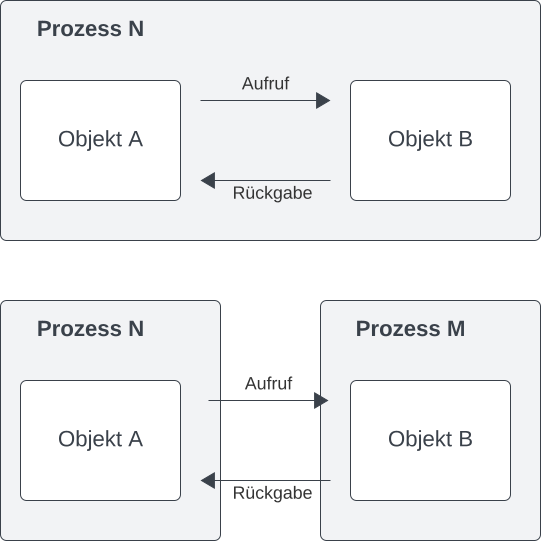
\includegraphics[scale=0.5]{chapters/fopt5/img/rmi/processcall}
    \caption{Zwei unterschiedliche Objekte in unterschiedlichen Aufrufsituationen. Im oberen Beispiel befinden sich die Objekte im selben Adressraum, im unteren Beispiel in unterschiedlichen Adressräumen - diese Situation kommt bei der Nutzung von RMI vor (Quelle: in Anlehnung an \cite[311 f., Abbildung 6.1 und 6.2]{Oec22})}
    \label{fig:processcall}
\end{figure}

\begin{figure}
    \centering
    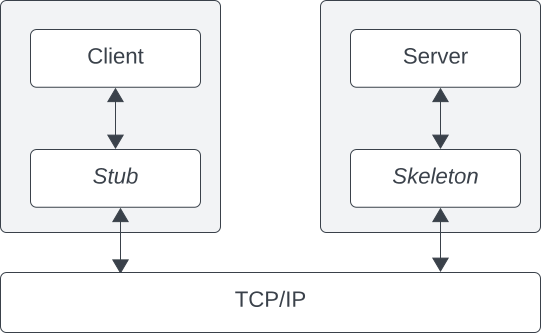
\includegraphics[scale=0.4]{chapters/fopt5/img/rmi/stubskeleton}
    \caption{Prinzip der Kommunikation zwischen RMI-Client und -Server. (Quelle: in Anlehnung an \cite[312, Bild 6.3]{Oec22})}
    \label{fig:stubskeleton}
\end{figure}


\begin{figure}
    \centering
    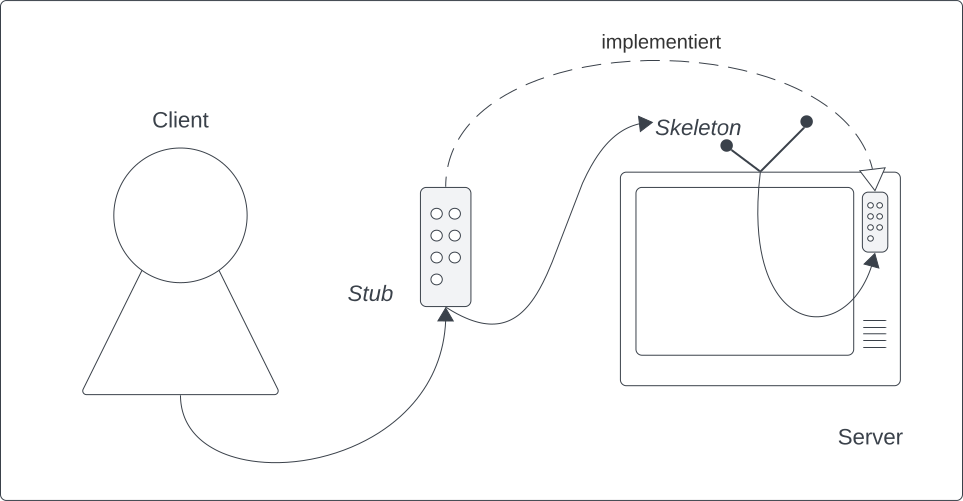
\includegraphics[scale=0.35]{chapters/fopt5/img/rmi/tv}
    \caption{Eine Illustration der im Lehrbuch verwendeten RMI-Metapher. Ein Client will ein entferntes Objekt (TV) bedienen. Hierzu verwendet er Methodenaufrufe, die vom Stub (Fernbedienung) weitergeleitet werden. Die Methoden werden vom Skeleton (Fensehantennen) an das Objekt auf dem Server weitergeleitet. Dieses Objekt sind in dem Beispiel die Knöpfe an dem Fernseher, die die gleichen Bedienfunktionen (``Schnittstelle``) wie die Fernbedienung haben. (Quelle: eigene)}
    \label{fig:tv}
\end{figure}

\noindent
Die \textbf{Transparenz} kommt für den Entwickler dadurch zustande, dass er nur Client und Server, nicht aber Stub und Skeleton programmieren muss.\\
$\rightarrow$ \textbf{Stub} wird automatisch erzeugt, das \texbf{Skeleton}-Objekt ist ein Programmteil, der in der \textbf{RMI}-Implementierung dabei ist und für alle Anwendungen verwendet werden kann.\\

\noindent
Die Entwicklung einer \textbf{RMI}-Anwendung erfolgt i.d.R. in folgenden Schritten\footnote{
s.a. ``An Overview of RMI Applications``: \url{https://docs.oracle.com/javase/tutorial/rmi/overview.html} - abgerufen 1.2.2024
}:

\begin{enumerate}
    \item\label{itm:intdef} \textbf{Schnittstelle definieren}\\
    \noindent
    Die Schnittstelle zwischen Client \& Server in Abhängigkeit von der Anwendung, die realisiert werden soll.\\
    \noindent
    Die Schnittstelle führt alle Methoden auf, die über \textbf{RMI} aufgerufen werden sollen.\\
    \noindent
    Die Schnittstelle muss aus \code{java.rmi.Remote} abgeleitet werden.\\
    \noindent
    Alle Methoden der Schnittstelle müssen mit \code{throws RemoteException} gekennzeichnet werden\footnote{
    s.a. ``2.4.1 The java.rmi.Remote Interface``: \url{https://docs.oracle.com/en/java/javase/21/docs/specs/rmi/objmodel.html#the-java.rmi.remote-interface} - abgerufen 1.2.2024
    }.

    \item \textbf{Schnittstelle implementieren}\\
    \noindent
    Es wird eine Klasse geschrieben, die die im ersten Schritt definierte Schnittstelle implementiert.\\
    \noindent
    Einem Objekt davon muss \ul{von außen über RMI} nutzbar sein - es muss exportiert werden können.
    Dazu kann die implementierende Klasse von \code{UnicastRemoteObject} abgeleitet werden.\\
    Es muss ein expliziter Konstruktor existieren, der mit \code{throws RemoteException} gekennzeichnet wird. \\
    $\rightarrow$ Es muss mindestens ein expliziter Standard-Konstruktor existieren, der diese Bedingung erfüllt\footnote{
    ansonsten wird vom Compiler ein Standard-Konstruktor zur Verfügung gestellt.
    Da dieser aber keine checked Exception in Form einer \textit{RemoteException} wirft, kommt es zu einem Compilerfehler.
    }

    \item \textbf{Server programmieren}\\
    \noindent
    Man erzeugt eines oder mehrere Objekte der in Schritt 2 implementierten Klasse und meldet diese unter einem beliebigen Namen bei der \textbf{RMI-Registry} an.

    \item \textbf{Client programmieren}\\
    \noindent
    Über die \textbf{RMI-Registry} (Serveradresse und Port müssen dem Client bekannt sein) beschafft sich der Client die in Schritt 3 registrieren Objekte, die als \textbf{Stub} an ihn weitergeleitet werden.\\
    \noindent
    Der Stub kann unter Berücksichtigung der in Schritt 1 definierten Schnittstelle so verwendet werden, als wäre es ein lokales Objekt\footnote{
    ``lokal`` im Sinne von gleicher Prozess / gleicher Adressraum.
    }.\\
    \noindent
    Die Methodenaufrufe werden dann letztendlich auf dem durch das in Schritt 2 definierte \textbf{RMI-Objekt} auf dem Server ausgeführt (Client $\rightarrow$ Stub $\rightarrow$ Skeleton $\rightarrow$ Server).

    \item \textbf{Anwendung übersetzen und ausführen}\\
    \noindent
    Alle Dateien werden kompiliert.
    Vor dem Starten des Programms ist darauf zu achten, dass auf dem Server die \textbf{RMI-Registry} gestartet wird - was aber auch aus dem Programm heraus geschehen kann.
\end{enumerate}

\section{Einführendes RMI-Beispiel}\label{sec:rmiintro}

Auch bei RMI-Implementierungen bei denen mehrere Clients gleichzeitig auf eine Objektinstanz zugreifen, ist (ggf. nach Anwendung) \code{synchronized} nötig, um ein Objekt für den gleichzeitigen Zugriff zu sperren.\\

\noindent
Sobald über \staticcode{java.rmi.Naming.rebind()} bzw. \staticcode{bind()}\footnote{
textit{bind()} wirft eine \textit{AlreadyBoundException}, falls in der RMI-Registry bereits ein Eintrag mit dem Namen existiert, \textit{rebind()} hingegen ersetzt einen ggf. breits existierenden Eintrag mit gleichem Namen.
} der Server gestartet wurde, wird ein Thread gestartet, der den Skeleton repräsentiert, und auf eingehende TCP-Verbindungen wartet.\\

\noindent
Der Client fragt vom Server über

\begin{minted}[mathescape,
    numbersep=5pt,
    gobble=2,
    frame=none,
    framesep=2mm]{java}
    java.rmi.Naming.lookup("rmi://serveradresse/bindingname");
\end{minted}\\

\noindent
das Objekt ab, auf das er zugreifen möchte, und bekommt dann ein Objekt vom Typ \code{java.rmi.Remote} zurück.\\
Das Objekt muss noch zu dem Typen gecasted werden, der in ``Schnittstelle definieren`` in Punkt~\ref{itm:intdef} (s. vorheriger Abschnitt) implementiert wurde, um entsprechende Methoden der implementierten Schnittstelle aufrufen zu können - \ul{das über }\code{lookup()}\ul{ zurückgegebene Objekt ist das \textbf{Stub-Objekt}}.\\

\noindent
Bevor der Server auf dem entsprechenden Rechner gestartet wird, muss auf diesem Rechner über die Konsole noch \code{rmiregistry} aufgerufen werden, damit die \textbf{Registry} zur Verfügung steht, sofern das nicht wie im folgenden Beispiel über das Programm geschieht.
Das Listing zeigt die Implementierung für einen einfachen Echo-Server\footnote{
``Echo Protocol``: \url{https://en.wikipedia.org/wiki/Echo_Protocol} - abgerufen 2.2.2024
}.\\
Die RMI-Registry wird hierbei ebenfalls über das Programm gestartet.
\begin{minted}[mathescape,
linenos,
numbersep=5pt,
gobble=2,
fontsize=\small,
frame=lines,
framesep=2mm]{java}
    public class RMIDemo {

        interface Echo extends Remote {
            String echo(String msg) throws RemoteException;
        }

        static class EchoImpl extends UnicastRemoteObject implements Echo {

            public EchoImpl() throws RemoteException{}

            @Override
            public String echo(String msg) throws RemoteException {
                return msg;
            }
        }

        public static void main(String[] args) {
            if (args.length == 0) { // Server
                try {
                    Registry registry = LocateRegistry.createRegistry(1099);
                    registry.rebind("echo", new EchoImpl());
                } catch (RemoteException e) {
                    System.err.println("[registry] " + e);
                }
                return; //Thread is started, it's okay to leave main() at this point.
            }
            // client
            try {
                Remote stub = Naming.lookup("rmi://localhost:1099/echo");
                Echo echo = (Echo) stub;
                System.out.println(echo.echo(args[0]));
            } catch (NotBoundException | MalformedURLException | RemoteException e) {
                System.err.println("[client] " + e);
            }
        }
    }
\end{minted}

\begin{tcolorbox}[enlarge top by=0.5cm,enlarge bottom by=0.5cm]
    RMI-Methodenaufrufe sind blocking, auch wenn der Rückgabetyp für die aufgerufene Methoden mit \code{void}-deklariert wurde.\\

    \blockquote[{``3.1 Stubs and Skeletons``: \url{https://docs.oracle.com/en/java/javase/21/docs/specs/rmi/arch.html} - abgerufen 2.2.2024 (Hervorherbungen eigene)}]{
        When a stub's method is invoked, it does the following:
        \begin{itemize}
            \item initiates a connection with the remote JVM containing the remote object,
            \item marshals (writes and transmits) the parameters to the remote JVM,
            \item \textbf{waits for the result of the method invocation},
            \item \textbf{unmarshals (reads) the return value or exception returned}, and
            \item returns the value to the caller.
        \end{itemize}

    }
\end{tcolorbox}

\subsection{RMI-Client mit grafischer Benutzeroberfläche}

In Listing 6.5 (\cite[320]{Oec22}) wird bei jedem Buttonclick ein neuer Thread gestartet.
Die gestarteten Threads können unterschiedlich schnell ablaufen, und somit zu unerwarteten Ergebnissen führen:

\blockquote[{\cite[323]{Oec22}}]{
[...] man wird vermutlich davon ausgehen, dass der angezeigte Zählerwert immer derjenige ist, der aus der eigenen zuletzt angestoßenen Aktion resultiert.
    Aber dies muss nicht in jedem Fall so sein.
}

Als Lösung könnte man die ankommenden Aufträge durch einen einzigen Thread ausführen lassen, indem die Aktionen {bspw.} in eine Warteschlange eingereiht werden (vgl.~\cite[323]{Oec22}).

\newpage
In dem o.a. Listing wird das Functional Interface \code{Consumer}\footnote{
`´Interface Consumer<T>``: \url{https://docs.oracle.com/en/java/javase/21/docs/api/java.base/java/util/function/Consumer.html} - abgerufen 2.2.2024
} verwendet.
Folgendes Beispiel stellt die Verwendung in vereinfachter Form nochmal dar:


\begin{minted}[mathescape,
    linenos,
    numbersep=5pt,
    gobble=2,
    fontsize=\small,
    frame=lines,
    framesep=2mm]{java}
    public class ConsumerDemo {
        interface Supplier<T> {
            T execute();
        }

        public <T> void asyncCall(Supplier<T> s, Consumer<T> c) {
            startThread(s, c);
        }

        public <T> void startThread(Supplier<T> s, Consumer<T> c) {
            Thread t = new Thread(() -> c.accept(s.execute()));
            t.start();
        }

        public static void main(String[] args) {
            ConsumerDemo cd = new ConsumerDemo();
            cd.asyncCall(
                () -> Math.random() * 100,
                (r) -> System.out.println("Done: " + r)
            );
        }
    }
\end{minted}\\

\subsection{RMI-Registry}

\code{java.rmi.Naming} stellt die Methode \staticcode{bind()} zur Verfügung - wenn die Methode aufgerufen wird, und der Name schon vergeben (``gebunden``) ist, wird eine \code{AlreadyBoundException} geworfen; für ein \textit{rebinding} müsste die \textbf{RMI-Registry} neugestartet werden; aus dem Grund kann man \staticcode{rebind()} verwenden.\\
Wenn ein Server herunterfährt, sollte man auch mittels \staticcode{unbind()} die von ihm vorher registrierten RMI-Objekte wieder abmelden.

\begin{tcolorbox}[enlarge top by=0.5cm,enlarge bottom by=0.5cm]
    \code{bind()}, \code{rebind()} und \code{unbind()}, ruft der Server auf, der sich auf dem gleichen Rechner befinden muss wie die \textbf{Registry}.\\
    \noindent
    \code{lookup()} und \code{list()} ruft i.d.R. der Client auf, der auf einem beliebigen Rechner laufen kann.
\end{tcolorbox}

\noindent
Eine weitere statische Methode ist \staticcode{list():String[]}, die einem ein Feld mit allen Einträgen der Registry zurückliefert.\\

\noindent
Die Kommunikation zwischen \ul{Client und Server}, \ul{Client und Registry} sowie \ul{Server und Registry} findet über \textbf{TCP-Sockets} statt.\\

\noindent
Die \textbf{Registry} startet standardmäßig auf Port $1099$.\\

\noindent
Ein Server startet auf einer beliebigen freien Portnummer; während der Registrierung werden einem Objekt weitere Informationen zugeordnet, wie Portnummer und eine \textit{Objekt-Id-Kennung}, damit man das Objekt erreichen kann.\\
Wenn der Client mittels \staticcode{java.rmi.Naming.lookup(name:String)} einen Eintrag aus der Registry anfordert, enthält das zurückgegebene Objekt diese Informationen, und der Client kann diese Informationen zur Verbindungsherstellung nutzen.

\begin{tcolorbox}[enlarge top by=0.5cm,enlarge bottom by=0.5cm]
    Ein Server kann mehrere Objekte beherbergen, die alle unter ein und derselben Portnummer erreichbar sind (vgl.~\cite[324]{Oec22}).
\end{tcolorbox}

\begin{figure}
    \centering
    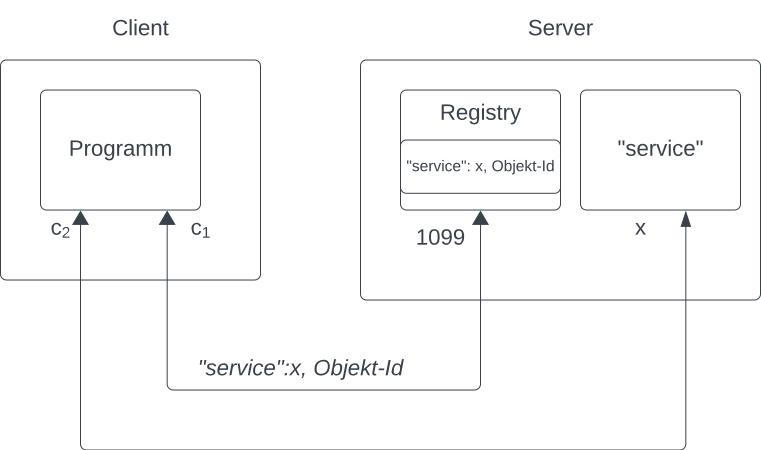
\includegraphics[scale=0.5]{chapters/fopt5/img/rmi/registry}
    \caption{Ein Client fragt den Eintrag der Registry für ``service`` ab und erhält über den Port des Client-Rechners $c_1$ die Erreichbarkeitsinformationen, die u.a. aus einer Portnummer $x$ und einer Objekt-Kennung bestehen.
    Antworten auf seine Anfragen werden daraufhin an seinen Port $c_2$ gesendet. (Quelle: in Anlehnung an \cite[324, Bild 6.5]{Oec22})}
    \label{fig:registry}
\end{figure}

Die \textbf{Registry} lässt sich auch aus dem Programm heraus starten\footnote{
``Class LocateRegistry``: \url{https://docs.oracle.com/en/java/javase/21/docs/api/java.rmi/java/rmi/registry/LocateRegistry.html} - abgerufen 2.2.2024
}:

\begin{minted}[mathescape,
    numbersep=5pt,
    gobble=2,
    frame=none,
    framesep=2mm]{java}
    java.rmi.registry.LocateRegistry.createRegistry(port:int):Registry
\end{minted}\\

\noindent
Der zurückgegebene Typ implementiert \code{java.rmi.registry.Registry} und besitzt dieselben Methoden wie \code{java.rmi.Naming}\footnote{was aber nicht heißt, dass \textit{Naming} auch \textit{Registry} implementiert - die Methoden von \textit{Naming} sind allesamt statisch.
}.\\
$\rightarrow$ Entweder wird die Registry nur in einem Server gestartet, oder weitere Registries müssen eigene, unterschiedliche Portnummern enthalten.

\subsection*{Eigene Notizen}

Länger andauernde Aufträge an ein Remote-Objekt sollten über Threads realisiert werden.\\

\noindent
Muss eine UI während / infolgedessen aktualisiert werden, sollte diese UI-Aktualisierung über \code{javafx.application.Platform.runLater()} stattfinden (\textbf{JavaFX Application Thread}).


\section{Parallelität bei RMI-Methodenaufrufen}\label{sec:rmiparallel}

Ein \textbf{Skeleton} ist ein paralleler \textbf{TCP-Server} (vgl.\cite[329]{, Oec22}).

\begin{tcolorbox}[enlarge top by=0.5cm,enlarge bottom by=0.5cm]
    Identität und Gleichheit von zwei \textbf{Stubs}:\\
    \noindent
    Rückgabewert von \code{Naming.lookup(...)} führt bei Objektvergleich mittels $==$zu \code{false}, wenn ein Stub für ein und denselben Namen zweimal angefordert wird, \code{equals()} hingegen zu \code{true}.\\

    $\rightarrow$ \textbf{Stub-Objekte} sind in diesem Fall nicht ``identisch``, aber wenn sie auf dasselbe \textbf{RMI-Objekt} zeigen, werden sie als ``gleich`` betrachtet.\\

    ``Zwei Stub-Objekte sind genau dann gleich, wenn sie eine Referenz auf dasselbe Objekt in der Ferne repräsentieren.`` (\cite[347]{Oec22})
\end{tcolorbox}\\

\noindent
Wird ein \textbf{Stub} angefordert, der eine asynchrone Operation ausführt, und dieser Stub wird in einen Thread ausgelagert, verhält sich der Stub \textit{intelligent}:

\begin{itemize}
    \item \ul{wenn mehrere Threads erzeugt werden}, und ``parallel`` gearbeitet wird, werden die Operationen auch parallel ausgeführt, und zwar indem mehrere Verbindungen aufgebaut werden (dadurch werden auf Server-Seite mehrere Threads erzeugt).
    \item wird auf Client-Seite keine parallele Ausführung durch die Erzeugung von Threads erzwungen, findet die Abarbeitung der Operation(en) sequentiell statt, es wird dann auch nur eine Verbindung dafür aufgebaut.
    \item ein einzelner Stub ist also auch dazu in der Lage, parallele Aufrufe auf dem Server zu erzeugen
\end{itemize}

\begin{tcolorbox}[enlarge top by=0.5cm,enlarge bottom by=0.5cm]
    Methodenaufrufe auf ein RMI-Objekt finden parallel statt durch mehrere Clients - beim Zugriff auf gemeinsame Daten muss entsprechend synchronisiert werden\footnote{
        s.a. ``3.2 Thread Usage in Remote Method Invocations``: Die Spezifikationen scheinen hier keinen Hinweis darauf zu geben, dass es eine Garantie für die Threads gibt. Steht das im Widerspruch zu der Aussage im Buch (\cite[330]{Oec22})? \url{https://docs.oracle.com/en/java/javase/21/docs/specs/rmi/arch.html#thread-usage-in-remote-method-invocations} - abgerufen 2.2.2024
    }.
\end{tcolorbox}

\begin{tcolorbox}[colback=red!20,color=white,title=Anmerkung]
    Die Spezifikationen unter ``3.2 Thread Usage in Remote Method Invocations``\footnote{
        \url{https://docs.oracle.com/en/java/javase/21/docs/specs/rmi/arch.html#thread-usage-in-remote-method-invocations} - abgerufen 2.2.2024
    } geben keinen Hinweis darauf, dass es eine Garantie für die Threads gibt, im Gegensatz zu~\cite[330]{Oec22}.
\end{tcolorbox}

\section{Wertübergabe für Parameter und Rückgabewerte}

Bei \textbf{RMO} können Objektparameter oder Objektrückgabewerte als \textbf{Wert} oder \textbf{Referenz} übergeben werden.\\

\noindent
Bei der Übergabe als Wert wird eine Kopie des Objektes erzeugt, und zwar rekursiv bei gleichzeitiger Vermeidung von Zyklen.\\

\noindent
Diese Kopie wird dann auf dem Server in der entsprechenden Methode aufgerufen:

\begin{tcolorbox}[enlarge top by=0.5cm,enlarge bottom by=0.5cm]
    Damit ein Objekt auf einen Server übertragen werden kann, muss es \code{java.io.Serializable} implementieren.
\end{tcolorbox}

\begin{itemize}
    \item wird das Objekt auf dem Server geändert, ändert sich nur \ul{dieses} Objekt auf dem Server, nicht aber das auf dem Client.
    \item \ul{als Rückgabewert} kann das geänderte Objekt aber vom Client verwendet werden
\end{itemize}

Datenstrukturen werden unter Verwendung von \code{java.io.Serializable} serialisiert {bzw.} deserialisiert; Objekte, die als ``Foge von Bytes`` serialisiert werden sollen, müssen dabei \code{java.io.Serializable} implementieren  - das gilt auch für die Objekte, die mit dem zu serialisierenden Objekt assoziiert sind (vgl.~\cite[332]{Oec22}).\\

\noindent
Bei \textbf{RMI} findet die Serialisierung automatisch statt; möchte man {bspw.} ein Objekt serialisieren und in eine Datei schreiben, muss man die Logik zum Speichern/Lesen des Objektes selber implementieren\footnote{
auch wenn das Beispiel nicht viel Code enthält, sollte klar sein, dass das (De)Serialisieren bei RMI automatisch geschieht und bei Abfrage des Rückgabewerts/ Übergabeparameters bereits erfolgt ist, ohne dass zusätzliche Methoden aufgerufen werden müssen.
}, wie folgendes Beispiel zeigt:\\

\begin{minted}[mathescape,
    numbersep=5pt,
    gobble=2,
    frame=none,
    framesep=2mm]{java}

    // schreiben
    FileOutputStream fos = new FileOutputStream(fileName);
    ObjectOutputStream output = new ObjectOutputStream(fos);
    // hier findet das serialisieren statt
    output.writeObject(obj);
    output.flush();

    //lesen
    FileInputStream fis = new FileInputStream(fileName);
    ObjectInputStream input = new ObjectInputStream(fis);
    // hier findet das de-serialisieren statt
    ConcreteObject obj = (ConcreteObject)input.readObject();
\end{minted}\\

\noindent
Im Wesentliche wird bei der Serialisierung der Zustand eines Objektes gespeichert, was vor allem durch die aktuellen Werte der Attribute des Objektes beschrieben wird.\\

\noindent
Attribute, die bei der Serialisierung nicht berücksichtigt werden sollen, können durch den Feld-Modifier \code{transient} entsprechend gekennzeichnet werden\footnote{
vgl. ``8.3.1.3. transient Fields`` \url{https://docs.oracle.com/javase/specs/jls/se21/html/jls-8.html#jls-8.3.1.3} - abgerufen 2.2.2024
}.


\begin{tcolorbox}[enlarge top by=0.5cm,enlarge bottom by=0.5cm]
    Ein Objekt wird als Wert übergeben, wenn es serialisierbar ist und nicht exportiert ist.
\end{tcolorbox}


\section{Referenzübergabe für Parameter und Rückgabewerte}

Bei \textbf{RMI} werden Parameter und Rückgabewerte entweder als Wert oder als Referenz übergeben.\\

\noindent
Als \textbf{Wert} i.d.R. nur, wenn eine Klasse \code{Serializable} implementiert, ansonsten hat die \textbf{Referenzübergabe} Vorrang, falls ein Objekt einer Klasse \textbf{exportiert} ist (bspw. weil seine Klasse von \code{UnicastRemoteObject} abgeleitet ist).

\begin{tcolorbox}[enlarge top by=0.5cm,enlarge bottom by=0.5cm]
    RMI-Objekte implementieren die \code{Remote}-Schnittstelle und sind aus \code{UnicastRemoteObject} abgeleitet.
\end{tcolorbox}\\

\noindent
Für ein Objekt, das bei \textbf{RMI} als Referenz übergeben wird, wird ein \textbf{Stub} erzeugt, hierzu muss aber nicht extra das betreffende Objekt in einer Registry registriert sein - der Server erhält das \code{Stub}-Objekt nicht über die Registry!\\

\noindent
Eine Übergabe als Referenz ist bspw. dann sinnvoll/ notwendig, wenn der Server auf dem Client Daten ändern muss\footnote{als Beispiel die in Abschnitt 6.5 des Buches vorgestellte Chat-Anwendung - der Server ruft die \textbf{print}-Methode der Clients auf, Clients aktualisieren daraufhin ihr UI mit dem Übergabeparameter... (vgl.~\cite[Listing 6.22, Listing 6.24]{Oec22})}.\\

\noindent
Damit eine Übergabe als Referenz funktioniert, muss das übergebende Objekt vom Typ \code{Remote} (und exportiert) sein.\\

\noindent
Werden \code{UnicastRemoteObjekte} genutzt, erstellen diese zur \textbf{TCP}-Kommunikation Threads.
Deshalb sollte darauf geachtet werden, dass diese Threads beendet sind, bspw. durch einen Aufruf von \code{System.exit(0)}, wenn es zu einem ``kontrollierten`` Programmende kommt\footnote{s. \cite[352]{Oec22}; außerdem ``Shutdown Sequence``: \url{https://docs.oracle.com/en/java/javase/21/docs/api/java.base/java/lang/Runtime.html#shutdown} - abgerufen 2.2.2024
}.

\begin{tcolorbox}[enlarge top by=0.5cm,enlarge bottom by=0.5cm]
    \item Ein Objekt, das eine \textbf{RMI}-Schnittstelle implementiert und von \code{UnicastRemotObject} abgeleitet ist und \textbf{serialisierbar} ist, wird trotzdem als \textbf{Referenz} übergeben.\\

    \noindent
    \textbf{Referenzübergabe} hat Vorrang vor \textbf{Wertübergabe}.
\end{tcolorbox}

\subsection*{Eigene Notizen}

\noindent
Eine \code{ArrayList} nutzt in ihren Methoden bei Objekten \code{equals} zum Vergleich der enthaltenen Elemente\footnote{
    s. \url{https://docs.oracle.com/en/java/javase/21/docs/api/java.base/java/util/ArrayList.html#equals(java.lang.Object)} - abgerufen 2.2.2024
}.\\

\noindent
Über einen \code{Iterator} können bedenkenlos Objekte entfernt werden, ohne, dass es zu einer \code{ConcurrentModificationException} kommt\footnote{ein Iterator kennt \textit{remove()}, aber kein \textit{add()}. S. \url{https://docs.oracle.com/en/java/javase/21/docs/api/java.base/java/util/Iterator.html#remove()} - abgerufen 2.2.2024}.\\


\noindent
Chatbeispiel: Dem Abmelden von Clients sollte genug Zeit eingeräumt werden - funktioniert das Abmelden nicht richtig, entfernt der Server die fehlerhaften Clients allerdings ohnehin wegen der abgefangenen Exception - s. \cite[345, Listing 6.22]{Oec22}.


\section{Transformation lokaler in verteilte Anwendungen}

Um eine lokale Anwendung in eine RMI-Anwendung zu überführen, wird die \textit{passive Klasse} (s. Abschnitt~\ref{subsec:syncsummary}) als Remote-Interface implementiert und von \code{UnicastRemoteObject} abgeleitet.
Daraufhin können Objekte davon als \textbf{RMI-Objekte} von einem Server in der \textbf{RMI-Registry} registriert werden.\\

\noindent
Der Server wartet dann passiv auf Aufrufe durch die \textbf{RMI-Clients}, also Objekte \textit{aktiver Klassen}, die über \code{Naming.lookup()} Zugriffe auf die vom Server zur Verfügung gestellten \code{RMI-Objekte} erhalten.\\

\noindent
Man muss berücksichtigen, dass bei der Entwicklung von RMI-Anwendungen, die mit Sperren arbeiten, die Sperre nicht auf den Objekten auf dem lokalen Rechner gesetzt werden, sondern auf den entfernten Objekten. \\
Wie in Abschnitt~\ref{sec:rmiintro} festgestellt wurde, sind Methodenaufrufe auf RMI-Objekte \textit{blocking}: Ruft also ein Client-Thread auf einem entfernten Objekt eine Methode auf, die den Aufrufer bspw. in eine Warteschlange einfügt, dann ist der Client ebenso lange blockiert wie das in der Warteschlange befindliche Stellvertreterobjekt\footnote{
zu ``Stellvertreterobjekte`` s.a. \url{https://openbook.rheinwerk-verlag.de/java8/14_003.html#u14.3.3} - abgerufen 5.2.2024
}.\\
Ist nun für die RMI-Kommunikation über \begin{center}\code{sun.rmi.transport.tcp.responseTimeout}\end{center} ein Timeout gesetzt, kann es vorkommen, dass aufgrund länger andauernder Prozesse eine \code{java.rmi.RemoteException} geworfen wird:

\blockquote[{``sun.rmi.transport.tcp.responseTimeout``: \url{https://docs.oracle.com/javase/8/docs/technotes/guides/rmi/sunrmiproperties.html} - abgerufen 5.2.2024, Hervorhebungen entfernt}]{
    The value of this property represents the length of time (in milliseconds) that the client-side Java RMI runtime will use as a socket read timeout on an established JRMP connection when reading response data for a remote method invocation. Therefore, this property can be used to impose a timeout on waiting for the results of remote invocations; if this timeout expires, the associated invocation will fail with a java.rmi.RemoteException. Setting this property should be done with due consideration, however, because it effectively places an upper bound on the allowed duration of any successful outgoing remote invocation. The maximum value is Integer.MAX\_VALUE, and a value of zero indicates an infinite timeout. The default value is zero (no timeout).
}\\

\noindent
Auf CLient-Seite sollte dies entsprechend berücksichtigt werden.\\
Per default ist dieser Timeout-Wert nicht gesetzt (vgl. \cite[359]{Oec22}).

\subsection{Verteilte MVP-Anwendung}

Eine MVP-Anwendung kann ohne weiteres in eine RMI-Anwendung überführt werden.\\

\noindent
Hierfür ist es wichtig, die Verantwortlichkeiten der einzelnen Bestandteile der Anwendung auszumachen - i.d.R. ist das \textbf{Model} der Bestandteil, der als entferntes RMI-Objekt über einen Server den Clients der Anwendung zur Verfügung gestellt wird.\\

Der \textbf{Presenter} enthält eine Referenz auf das Model.
Gleichzeitig kann das Model mit dem Presenter kommunizieren, damit eine Aktualisierung der Daten in allen angeschlossenen Clients - und damit allen Views - passieren kann.\\

\noindent
In dem folgenden Beispiel wird ein einfaches Model implementiert, das in einem Thread jede Sekunde ein \textit{increment} von \textit{value} vornimmt.\\
Die dem Model übergebenen \code{Presenter}-Objekte werden als Referenz übergeben; Änderungen sind folglich in allen so angeschlossenen Clients sichtbar.\\
Wird hingegen die \code{PresenterImpl}-Klasse so abgeändert, dass sie \code{Serializable} implementiert und nicht mehr von \code{UnicastRemoteObject} ableitet\footnote{
aufgrund der Assoziation zu {\textit{View}} muss auch diese Klasse \textit{Serializable} implementieren, sonst kommt es zu einer {\textit{java.rmi.MarshalException}}
}, werden Kopien der Presenter-Objekte an das RMI-Objekt übergeben: Wenn die Liste nun in \code{increment()} durchlaufen wird, finden die Konsolenausgabe auf dem Rechner statt, auf dem der Server läuft - die Clients werden nicht informiert.

\begin{minted}[mathescape,
    linenos,
    numbersep=5pt,
    gobble=2,
    fontsize=\small,
    frame=lines,
    framesep=2mm]{java}
    public class RmiMvpDemo {
        interface Presenter extends Remote {
            void setView(View v) throws RemoteException;
            void updateView(int value) throws RemoteException;
        }

        interface Model extends Remote {
            void increment() throws RemoteException;
            void addClient(Presenter client) throws RemoteException;
        }
        static class PresenterImpl extends UnicastRemoteObject implements Presenter {
            private View view;
            public PresenterImpl() throws RemoteException{}
            public void setView(View v){
                this.view = v;
            }
            public void updateView(int value){
                this.view.update(value);
            }
        }
        static class ModelImpl extends UnicastRemoteObject implements Model {
            private List<Presenter> clients = new ArrayList<>();
            private int value = 0;
            public ModelImpl() throws RemoteException {
                Thread t1 = new Thread(()-> {
                    while (true) {
                        try {
                            Thread.sleep(1000);
                            increment();
                        } catch (RemoteException | InterruptedException ignored) {
                        }
                    }
                });

                t1.start();
            }
            public synchronized void addClient(Presenter c) throws RemoteException {
                clients.add(c);
            }
            public synchronized void increment() throws RemoteException {
                value++;
                System.out.println(value);
                for (Presenter client: clients) {
                    client.updateView(value);
                }
            }
        }
        static class View {
            private final String name;
            public View(Presenter p, String n) throws RemoteException {
                this.name = n;
                p.setView(this);
            }
            public void update(int value) {
                System.out.println("[client:" + name + "] update " + value);
            }
            public String toString() {
                return name;
            }
        }

        public static void main(String[] args)
            throws RemoteException, MalformedURLException, NotBoundException {
            if (args.length == 0) { // server
                System.out.println("starting Server...");
                ModelImpl counterModel = new ModelImpl();
                Registry r = LocateRegistry.createRegistry(1099);
                r.rebind("counterModel", counterModel);
            } else { // client, 1st arg is its displayname
                System.out.println("starting Client...");
                Model counterModel = (Model) Naming.lookup("counterModel");
                PresenterImpl presenter = new PresenterImpl();
                new View(presenter, args[0]);
                counterModel.addClient(presenter);
            }
        }
    }
\end{minted}\\

\section{Verteilte Anwendungen mit Sockets}

Eigenständige \codebf{Client-Server-Anwendungen} können auf 3 verschiedene Arten umgesetzt werden:

\begin{itemize}
    \item Socket-Programmierung (Socket: Schnittstelle für \textbf{UDP} / \textbf{TCP} \footnote{
    UDP: \textit{User Datagram Protocol}; TCP: \textit{Transmission Control Protocol}
    })
    \item \textbf{RMI} \textit{Remote Method Invocation}: Die Methode eines Objektes, das auf einem anderen Rechner liegt, kann von einem anderen entfernten Rechner aufgerufen werden; RMI basiert auf Sockets und stellt somit eine höhere Schnittstelle mit einem höheren Abstraktionsniveau dar
    \item \textbf{indirekte Kommunikation}: Nachrichten werden durch einen Vermittler von einem Sender zu einem Empfänger weitergeleitet
\end{itemize}


\subsection{Schichtenmodell}

\subsection*{Schicht 1 - (Physical Layer)}

Diese Schicht ist zuständig für die Übertragung von Datenblöcken zwischen zwei Rechnern, die direkt miteinander verbunden sind (genauso wie \textbf{Schicht 2}).\\
Sie ist zuständig für die Übertragung einzelner Bits und wird deshalb auch \textbx{Bitübertragungsschicht} genannt.

\subsection*{Schicht 2 - DataLink Layer}

Wie Schicht 1 ist auch diese Schicht zuständig für die Übertragung von Datenblöcken zwischen zwei direkt miteinander verbundenen Rechnern.\\

Die Schicht hat die Aufgabe, einzelne Bits zu einem Datenblock in einem bestimmten Format zusammenzufassen.\\
$\rightarrow$ bestimmte Informationen wie z.B. Adressen haben eine bestimmte Struktur und Bitlänge und stehen an bestimmten Stellen in einem Datenblock.\\

\noindent
Bei lokalen Netzen wie {bspw.} Ethernet hat die \textbf{Leitungsschicht} durch das gemeinsame Medium noch weitere Funktionen: Sie garantiert, dass immer nur höchstens eine Station sendet, außerdem werden durch sie die angeschlossenen Rechner korrekt adressiert\footnote{
``Bei einer Punkt-zu-Punkt-Leitung kann eine empfangene Station davon ausgehen, dass die ankommenden Daten für sie bestimmt sind, bei einem gemeinsamen Medium dagegen nicht.``~\cite[257]{Oec22}
}

\begin{tcolorbox}
    Schicht 1 und 2 werden über Hardware ({bspw.} Ethernet-Adapter) und entsprechende Treiber im Betriebssystem realisiert.
\end{tcolorbox}

\noindent
Die beiden Funktionen (eine Station sendet, korrekte Adressierung) werden als \textbf{Medium Access Control} (\textit{MAC}) bezeichnet und bilden eine Teilschicht innerhalb der Leitungsschicht (\textit{DataLink Layer}).\\
Die entsprechenden Adressen heissen deshalb \textit{MAC-Adressen}.

\subsection*{Schicht 3}
Schicht 3 ist die \textbf{Vermittlungsschicht} (\textbf{Network Layer}), hier befindet sich das \textbf{IP-Protokoll}, über das Rechner verbunden werden, die an verschiedene Netze mit unterschiedlichen Netztechnologien angeschlossen sind.\\

\noindent
Jeder Netzanschluss enthält eine eindeutige \textbf{IP-Adresse}.\\
Die Schicht sorgt für eine einheitliche, strukturierte und weltweit eindeutige Adressierung (vgl.~\cite[258]{Oec22}).\\

\noindent
Über das IP-Protokoll werden Datenpakete über verschiedene Netze weitergeleitet, bis sie beim Zielrechner ankommen.\\

\noindent
Es kann durchaus vorkommen, dass Datenpakete verlorengehen, oder verzögert und/oder in unterschiedlicher Reihenfolge beim Empfänger eintreffen.


\begin{tcolorbox}
    Schicht 3 und 4 sind i.d.R. Teil des Betriebssystemkerns.
\end{tcolorbox}

\subsection*{Schicht 4}
Schicht 4 ergänzt die Adressierung in Schicht 3 um \textit{Kontaktpunkte} durch \textbf{Portnummern}, und wird \textbf{Transportschicht} (\textbf{Transport Layer}) genannt.\\

\noindent
Zwei verbreitete Transportprotokolle sind \textbf{UDP} und \textbf{TCP};

\begin{itemize}
    \item \textbf{UDP} (\textit{User Datagram Protocol}) hat dieselbe Eigenschaften wie das IP-Protokoll und erweitert es um die Adressierung mit Portnummern.\\
    Es ist genauso   \textit{verbindungslos} und \textit{unzuverlässig}\footnote{
    es sind Verluste und Reihenfolgevertauschungen möglich.
    } wie das IP-Protokoll.
    \item \textbf{TCP} (\textit{Transmission Control Protocol}) behebt die Nachteile des IP-Protokolls: Die Empfänger müssen den Nachrichtenerhalt bestätigen\footnote{ \textbf{ACK},
    was wiederum von Sender-Seite überwacht wird; s.a. ``Transmission Control Protocol``: \url{https://en.wikipedia.org/wiki/Transmission_Control_Protocol} - abgerufen 30.01.2024
    }, ansonsten wird die Nachricht nochmals gesendet.
\end{itemize}


\subsection*{Schicht 5}
Schicht 5 ist die \textbf{Anwendungsschicht}\footnote{
    Im Buch werden 5 Schichten aufgeführt, das \textbf{OSI-Modell} hat in der \textit{Anwendungsorientierten Schicht} noch zwei zusätzliche Schichten, die \textbf{Session-Layer} und die \textbf{Presentation-Layer} (\url{https://en.wikipedia.org/wiki/OSI_model} - abgerufen 3.2.2024)
} (\textbf{Application Layer}), in ihr wird die Kommunikation der Anwendung abgewickelt (bspw. \textit{www}, \textit{email}, \textit{Videokonferenzen}).


\begin{tcolorbox}
    Schicht 5 wird über Anwendungsprozesse realisiert.
\end{tcolorbox}


\begin{figure}
    \centering
    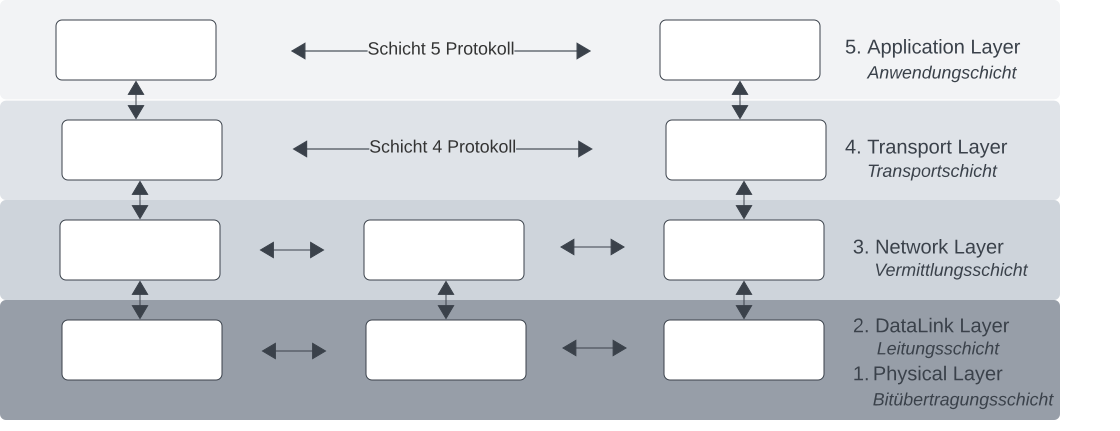
\includegraphics[width=16cm]{chapters/fopt5/img/layers}
    \caption{Skizze des Schichtenmodels. (Quelle: in Anlehnung an \cite[257, Bild 5.2]{Oec22})}
    \label{fig:layers}
\end{figure}


\subsection{IP-Adressen und DNS-Namen}

Ein Rechner kann mehrere Netzanschlüsse haben.\\

\noindent
Jeder dieser Netzanschlüsse ist eine weltweit eindeutige IP-Adresse zugeordnet.\\

\noindent
IP-Adressen können auch durch (Rechner-)Namen aufgelöst werden durch das \textbf{Domain Name System} (\textit{DNS}).\\

\noindent
Ein DNS-Name kann auch mehrere Aliase besitzen; dadurch, dass ein Rechner mehrere IP-Adressen haben kann (bspw. durch mehrere Netzanschlüsse) besteht so zwischen Rechnernamen und IP-Adressen eine $m:n$-Beziehung.


\subsection{Das Transportportprotokoll UDP}

Transportprotokolle existieren, damit mehrere Anwendungen, die über das Internet kommunizieren, gleichzeitig laufen und Daten untereinander austauschen können.\\

\noindent
Bei der Übertragung von Daten besitzt IP die Eigenschaften, dass Daten in unterschiedlicher Reihenfolge eintreffen können, was aus Anwendersicht problematisch ist; auf Anwendungsschicht könnte man hier Gegenmaßnahmen treffen, aber das würde bedeuten, die Gegenmaßnahmen in jeder Anwendung implementieren zu müssen - deshalb werden diese Problematiken in der \textbf{Transportschicht} über \textbf{Transportprotokolle} gelöst.\\

\noindent
\textbf{UDP} (\textbf{User Datagram Protocol}) ermöglicht die Kommunikation verschiedener Dienste gleichzeitig (spezifische Anwendung wird über Portnummer adressiert).\\

\noindent
Ein \textbf{Datagramm}\footnote{
Kunstwort abgeleitet aus\textit{Telegramm} (vgl.~\cite[260]{Oec22})
} bezeichnet eine Dateneinheit, die in ein IP-Paket gepackt und über das Netz verschickt wird.\\

\begin{tcolorbox}
\textbf{UDP} ist Nachrichtenorientiert.
\end{tcolorbox}

\noindent
Ein \textbf{UDP-Datagram} enthält neben der Zielportnummer auch die Quellportnummer, damit der Empfänger dem Sender antworten kann.

\noindent
UDP ist wie IP \textbf{verbindungslos} - es können \textit{Datagrammverluste} oder \textit{Reihenfolgevertauschungen} von Datagrammen vorkommen.\\

\noindent
UDP ist \textbf{datagrammorientiert}: Eine an das UDP-Protokoll übergebene Menge an Daten wird in ein Datagramm gepackt und über IP verschickt\\
$\rightarrow$ die Daten kommen als Einheit beim Empfänger an (entspricht dem Verhalten einer \textbf{Message Queue})


\subsection{Das Transportprotokoll TCP}

\textbf{TCP} ist ein Protokoll für genau zwei Partner, weshalb es nicht mit \textbf{Multicast} genutzt werden kann.\\

\noindent
\textbf{TCP} ist verbindungsorientiert, wobei der Verbindungsauf- und -abbau einen gewissen Aufwand erfordert\footnote{
    Wenn Datenverluste nicht hinnehmbar sind und wegen höherem Aufwand für die Verbindung trotzdem UDP verwendet wird, erweitert man die Anwendung entsprechend um Gegenmaßnahmen für den Datenverlust (vlg. \cite[261]{Oec22}).
}.

\noindent
\textbf{TCP} ist ein zuverlässiges Protokoll, es können keine Daten vertauscht oder verloren gehen, außerdem gibt es eine \textbf{Flusskontrolle} (zum Verhindern einer Überflutung des Empfängers mit Datenpaketen)\footnote{Empfangsbestätigung abwarten} und eine \textbf{Überlastkontrolle} (um eine Überlastung des Netzes zu verhindern)\footnote{informal: falls ein ACK ausbleibt, könnte der Sender versucht sein, ständig neue Pakete hinterherzuschicken, was zu einem Stau führen könnte. Siehe hierzu auch ``Modul 6: TCP-Überlastkontrolle``: \url{https://leischner.inf.h-brs.de/lehre/ikomm/ikomm06-ueberlastkontrolle.pdf} - abgerufen 30.01.2024}.\\

\noindent
\textbf{TCP} ist \textbf{datenstromorientiert} - der Empfänger erkennt an dem Datenstrom nicht, in welchen Portionen die Daten vom Sender geschickt wurden (entspricht dem Verhalten von \textbf{Pipes} (s. a. Abschnitt~\ref{sec:messagequeues})).


\setlength{\tabcolsep}{0.8em}
{\renewcommand{\arraystretch}{1.7}%
\begin{table}
[htbp]
    \centering

    \begin{tabular}{|l|l|}
        \toprule
        \hline
        \textbf{UDP} & \textbf{TCP}  \\
        \midrule
        \hline
        verbindungslos & verbindungsorientiert \\
        \hline
        unzuverlässig  & zuverlässig mit Fluss- und Überlastkontrolle \\
        \hline
        datagrammorientiert & datenstromorientiert \\
        \hline
        \bottomrule
    \end{tabular}

    \caption{Vergleich zwischen UDP und TCP. (Quelle: in Anlehnung an \cite[261, Tabelle 5.1]{Oec22})}

\end{table}










\newpage
\section*{Notizen}

\newpage
